% IEEE version (conference template IEEEtran 1.8b from CTAN, bare_conf.tex). Differs from the workshop version in
% paper/: no Network Decisions section, and QPSK and 64-QAM results with Fig. 5.
\documentclass[conference]{IEEEtran}
\IEEEoverridecommandlockouts
\usepackage{cite}
\usepackage{amsmath,amssymb,amsfonts}
\usepackage{graphicx}
\usepackage{textcomp}
\usepackage{xcolor}
\usepackage[hyphens]{url}
\newcommand{\red}[1]{\textcolor{red}{#1}}   % review notes; remove before submission

\begin{document}

\title{Stateful Neural Receivers: Amortizing Iterative Inference Across 5G NR Slots}

\author{
\IEEEauthorblockN{Hanze Lou}
\IEEEauthorblockA{Oakville Trafalgar Secondary School\\
louhansen811@gmail.com}
\and
\IEEEauthorblockN{Muhammad Sulaiman, Mohammad A. Salahuddin, Raouf Boutaba}
\IEEEauthorblockA{University of Waterloo\\
\{m4sulaim, mohammad.salahuddin, rboutaba\}@uwaterloo.ca}
}

\maketitle
\bstctlcite{IEEEexample:BSTcontrol}   % IEEE style: more than six authors -> first author et al.

\begin{abstract}
Neural receivers (NRXs) built from convolutional and graph neural network (CGNN) layers obtain their accuracy from iterative message passing, but in the real-time implementation of a state-of-the-art NRX for the 5G NR physical uplink shared channel (PUSCH), a 1\,ms latency budget admits only two of its eight iterations. We propose a stateful NRX that keeps a pilot memory, i.e., the least-squares channel estimates at the pilot positions of earlier slots of each user. A channel filter combines them with the current pilots; its weights are not trained but fitted per user by least squares on the memory itself, which requires neither channel statistics nor labels and adds no weights to the NRX. In $2\times 4$ multi-user MIMO simulations with QPSK, 16-QAM, and 64-QAM, the proposed NRX with two iterations requires 0.5 to 0.9\,dB less SNR than a stateless two-iteration NRX retrained on the same data and outperforms the released three-iteration NRX in all cases, with and without power control; with QPSK, it also outperforms the released eight-iteration NRX in all cases. It keeps most of its memory gain with phase jumps, frequency offsets, and TDD uplink slots, and it meets the 1\,ms real-time budget, which the three-iteration NRX exceeds.
\end{abstract}


% Index Terms are optional in the IEEE conference template; left out for space.

\section{Introduction}
Neural receivers (NRXs) replace channel estimation, equalization, and demapping with a single neural network trained on data~\cite{honkala2021deeprx}. Cammerer et al.~\cite{cammerer2023neural} brought this concept to multi-user multiple-input multiple-output (MU-MIMO) transmission over the 5G NR physical uplink shared channel (PUSCH), using convolutional and graph neural network (CGNN) layers that refine a state per user over several iterations. More iterations yield more reliable log-likelihood ratios (LLRs), but each iteration also adds latency. In the real-time implementation of this NRX, the 1\,ms budget admits only two of its eight iterations~\cite{wiesmayr2025realtime}. On our evaluation sequences, the cut to two iterations clearly raises the signal-to-noise ratio (SNR) required for a transport block error rate (TBLER) of 10\%, even when the NRX is retrained for two iterations.

Like other NRXs, this receiver processes each slot independently. Yet the channel of a user evolves continuously, so the pilots of earlier slots carry information about the current channel, which the receiver discards with each slot. Classical receivers exploit the temporal correlation of the channel by filtering pilots across time or by bundling the demodulation reference signals (DMRS) of several slots~\cite{hoeher1997wiener,3gpp38214}.

In this paper, we investigate whether an NRX can also leverage the pilots of earlier slots to substitute for iterations. We propose a stateful NRX that carries channel estimates across slots. It runs two CGNN iterations and keeps, for each user, a pilot memory with the least-squares (LS) channel estimates at the DMRS positions of up to seven previous transport blocks (TBs). A channel filter combines these entries with the current LS estimate before the first iteration. The filter coefficients are estimated online for each user by minimizing the prediction error of the historical channel estimates in the pilot memory, without prior channel statistics or ground-truth channel labels. The filter also selects how many historical estimates to use by how well they predict the current pilots, which mitigates outdated channel information after channel changes or scheduling gaps. We train the NRX on sequences of TBs rather than independent slots, starting from the released eight-iteration NRX, and add no trained weights. With two iterations, it recovers most of the accuracy that the cut from eight iterations costs.

In summary, our contributions are:
\begin{itemize}
\item We develop a stateful NRX with a pilot memory and a channel filter fitted on it without training.
\item We evaluate the proposed NRX in simulations of $2\times 4$ MU-MIMO with QPSK, 16-QAM, and 64-QAM over sequences of 64 slots, with and without power control: it clearly outperforms a stateless two-iteration NRX retrained on the same data and the released NRXs with up to three iterations, and performs close to the eight-iteration NRX.
\item It adds no CGNN weights, and our latency measurements with TensorRT show that it remains real-time capable, unlike the released three-iteration NRX.
\end{itemize}

\section{Related Work}
With TensorRT, the latency of the NRX of Cammerer et al.~\cite{cammerer2023neural} grows linearly with the number of iterations~\cite{wiesmayr2025realtime}. Site-specific fine-tuning lets a two-iteration receiver outperform an untuned eight-iteration receiver on over-the-air recordings at two indoor sites~\cite{baytekin2026site}, but it requires recorded site data and degrades performance on the original training distribution~\cite{wiesmayr2025realtime}. Other work reduces per-slot compute or model size through dynamic depth, low-rank adapters, quantization, lighter attention or blocks, and model-driven hybrids~\cite{yang2022dynamic,vanbolderik2024layerskip,vanbolderik2024mean,vanbolderik2026loren,yellapragada2026qat,yellapragada2026axial,kawai2025unified,fan2025choose,gupta2025lowcomplexity,gansekoele2025rpe,honkala2026eqdeeprx,abdollahpour2025mdx}, some at a cost in accuracy. Yet all of these methods process each slot from scratch, which Kawai and Koodli~\cite{kawai2025unified} name as a limitation.

Pooling pilots across time is an established way to improve channel estimates: Wiener filtering weights pilots by their time--frequency correlation~\cite{hoeher1997wiener}, Kalman tracking propagates an estimate and its error covariance~\cite{komninakis2002kalman}, and 5G NR Release~17 standardizes DMRS bundling over several PUSCH slots~\cite{3gpp38830,3gpp38214}, which requires a correlated channel and a continuous transmit phase. Their weights come from channel statistics or a channel model that a BS must estimate per user, and they stay the same when a user's channel changes. Learned predictors use recurrent, state-space and transformer models over past channel estimates~\cite{mattu2022deep,mohsin2025continual,luo2025cpmamba,lagona2026transformer,gizzini2021talstm} or set the parameters of a Kalman tracker~\cite{pratik2021hkf}, but target channel prediction or tracking, and none conditions a multi-user NRX on stored pilot history. Our filter instead fits its weights per user by least squares on the stored pilots, like an adaptive filter~\cite{haykin2002adaptive}, chooses on the current slot how many entries to use, and feeds an NRX; after a channel change, it stays ahead of a classical multi-slot estimator given each condition's statistics, which even falls 0.56\,dB behind its single-slot version.

Within learned receivers, earlier slots enter mainly through the weights: online schemes retrain on decoder-recovered labels, on symbol decisions, or when a drift test fires~\cite{fischer2022adaptive,finish2022symbol,uzlaner2025asynchronous}, or track a posterior over the weights~\cite{gusakov2026online}, and pay in label delay, compute, or error propagation~\cite{fischer2022adaptive,fan2025defined}. Time-averaged channel covariances~\cite{liu2026universal,wiesmayr2026impact} remain valid across scheduling gaps but do not supply the instantaneous channel. Kunde et al.~\cite{kunde2025transformers} show that a fixed-weight attention layer over past pilot pairs can represent the symbol posterior, but only with asymptotic theory and single-user, uncoded experiments.

% Fig. 1 belongs to the Receiver Design. It is defined here because a full-width figure appears at the top of
% the next page: the Receiver Design starts at the end of this page and refers to the figure there.
\begin{figure*}[t]
\centering
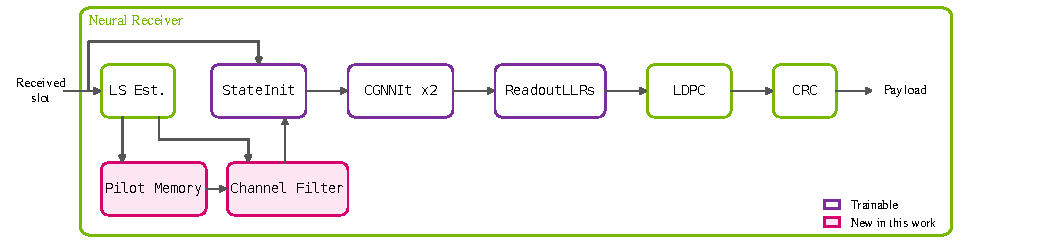
\includegraphics[width=\textwidth]{figures/receiver_architecture.pdf}
\caption{Proposed NRX for 5G NR PUSCH. The channel filter refines the LS estimate with the pilot memory before \texttt{StateInit}; its weights are fitted on the memory. The channel readout used only in training is not shown.}
\label{fig:architecture}
\end{figure*}

Despite these advances, no prior MU-MIMO NRX for 5G NR carries
channel estimates across slots to recover the accuracy lost to fewer
iterations. Unlike online adaptation, our receiver keeps its trained weights fixed and
stores only LS channel estimates, so it
needs no labels and no decoder feedback. Unlike DMRS bundling, it requires neither power
consistency nor phase continuity across the stored slots.

\section{Receiver Design}

\subsection{System Model}
We consider MU-MIMO uplink transmission from $U$ user equipments (UEs) to a base station (BS) with $B$ antennas over the 5G NR PUSCH~\cite{dahlman2020}. Each slot carries one TB per scheduled UE on an orthogonal frequency division multiplexing (OFDM) resource grid with $S$ subcarriers and $T=14$ OFDM symbols. The received signal on subcarrier $s$ and OFDM symbol $t$ is
\begin{equation}
\mathbf{y}_{s,t}=\sum_{u=1}^{U}\mathbf{h}_{s,t,u}\,x_{s,t,u}+\mathbf{n}_{s,t},
\end{equation}
where $\mathbf{h}_{s,t,u}\in\mathbb{C}^{B}$ is the effective channel of UE $u$ after its transmit beamforming, $x_{s,t,u}$ is its modulated symbol or pilot, and $\mathbf{n}_{s,t}\sim\mathcal{CN}(\mathbf{0},N_0\mathbf{I})$ is the noise. The receiver computes an LLR for each coded bit $b_{u,j}$, $j=1,2,\dots$, of the TB of each UE $u$. Given all received signals $\mathbf{Y}$ of the slot, we define the LLRs as logits, i.e., $\ell_{u,j}=\ln\big(\Pr(b_{u,j}=1\,|\,\mathbf{Y})/\Pr(b_{u,j}=0\,|\,\mathbf{Y})\big)$.

\subsection{Neural Receiver}
We build on the NRX architecture proposed by Cammerer et al.~\cite{cammerer2023neural} and extended by Wiesmayr et al.~\cite{wiesmayr2025realtime}, which comprises a state initialization layer (\texttt{StateInit}), a sequence of $N_{\mathrm{it}}$ CGNN blocks (\texttt{CGNNIt}), and an LLR readout layer (\texttt{ReadoutLLRs}). \texttt{StateInit} constructs an initial state for each UE from the received signal, the LS channel estimate, and a positional encoding of the distance to the nearest pilot. The CGNN blocks, each with its own weights, refine these states by message passing among UEs and convolutions over the resource grid, and \texttt{ReadoutLLRs} maps them to LLRs. A second readout, introduced by Wiesmayr et al., outputs refined channel estimates for an auxiliary loss in training. Following them, we call the configuration with $N_{\mathrm{it}}=8$, trained with a multi-loss that allows fewer iterations at inference, the \emph{Large NRX}. Within their 1\,ms budget, only $N_{\mathrm{it}}=2$ blocks can run.

The proposed stateful NRX, shown in Fig.~\ref{fig:architecture}, keeps this architecture with $N_{\mathrm{it}}=2$ and compensates for the fewer iterations with a pilot memory and a channel filter, neither of which adds trained weights. It thus has the $1.3\cdot 10^{5}$ trained weights of the Large NRX with $N_{\mathrm{it}}=2$, compared with $4.3\cdot 10^{5}$ for $N_{\mathrm{it}}=8$, excluding the training-only channel readout.

\subsection{Pilot Memory}
For each UE, the BS keeps the LS channel estimates at the DMRS positions of up to seven previous TBs, together with the slot index and the DMRS port of each TB. An entry is available as soon as the pilots of its slot are received, i.e., before the NRX processes that slot. Entries older than eight slots, i.e., 4\,ms at our 30\,kHz subcarrier spacing, are ignored, as they are likely outdated.

The memory is the only state kept across slots. As neither NRX outputs nor decoded bits or CRC outcomes enter it, no labels are needed and detection errors cannot propagate.

\subsection{Channel Filter}
The channel filter refines the LS estimate $\mathbf{h}^{(0)}_{p}\in\mathbb{C}^{B}$ at each DMRS position $p$, i.e., the subcarrier and OFDM symbol of an LS estimate, of the current TB of a UE. Let $\mathbf{h}^{(k)}_{p}$, $k\geq 1$, denote the LS estimate in the UE's $k$th newest entry. The filter first predicts $\mathbf{h}^{(0)}_{p}$ from the other estimates around $p$,
\begin{equation}
\tilde{\mathbf{h}}_{p}=\sum_{k=0}^{K}\sum_{q\in\mathcal{N}_{k}(p)}w_{k,q}\,\mathbf{h}^{(k)}_{q},
\label{eq:prediction}
\end{equation}
where $\mathcal{N}_{k}(p)$ contains, on each of the two DMRS symbols of TB $k$, the DMRS position closest to $p$ in frequency and its two neighbors, without $p$ itself for $k=0$, whose LS estimate is the one being predicted. The complex weights $w_{k,q}$ depend only on $k$ and on where $q$ lies relative to $p$, i.e., on its DMRS symbol and whether it is the closest, lower, or upper position; one set is used for all BS antennas and all positions on a DMRS symbol, and positions outside the band are left out.

The weights are not trained but fitted per UE on its memory. The fit emulates the prediction on earlier slots, for which the target is already stored. We use the three newest entries as targets. Each is treated as the current TB and predicted as in~\eqref{eq:prediction} from its own neighboring positions and from the entries before it, at the same slot offsets as in the actual prediction. The weights minimize the squared error of these predictions in the least-squares sense, with a regularization of $10^{-3}$ times the mean power of the estimates. As the noise of a predicted LS estimate is independent of the estimates it is predicted from, the weights also minimize, in expectation, the error relative to the true channel, as long as the channel and noise statistics do not change up to the current TB. The fit thus needs neither channel statistics nor labels and adapts to each UE's Doppler and delay spread. It only uses TBs received before the current slot, so the weights are computed before that slot arrives. For 132 physical resource blocks (PRBs) and $K=4$, 29 weights per DMRS symbol are fitted on $4.8\cdot 10^{3}$ LS estimates.

Since outdated entries carry little information about the current channel, we fit the weights for each $K\in\{0,\dots,4\}$, where $K=0$ uses the neighboring positions of the same TB only, and select, per DMRS symbol, the $K$ with the smallest mean squared difference $\sigma_{K}^{2}$ between $\tilde{\mathbf{h}}_{p}$ and $\mathbf{h}^{(0)}_{p}$ in the current TB. After a channel change or a scheduling gap, the filter thus leaves out the entries that no longer predict the channel. Since $\sigma_{K}^{2}$ is the sum of the error variance of the prediction and the known noise variance $\sigma_{\mathrm{LS}}^{2}$ of the LS estimate, both are combined by their error variances,
\begin{equation}
\hat{\mathbf{h}}_{p}=\mathbf{h}^{(0)}_{p}+\min\!\left\{1,\frac{\sigma_{\mathrm{LS}}^{2}}{\sigma_{K}^{2}}\right\}\left(\tilde{\mathbf{h}}_{p}-\mathbf{h}^{(0)}_{p}\right).
\end{equation}

Between the DMRS positions, the Large NRX holds the LS estimate of the nearest pilot. We instead apply a first-order model to the resource elements nearest to $p$, with slopes from the difference of $\hat{\mathbf{h}}_{p}$ to the DMRS position on the other DMRS symbol and from the difference between the frequency neighbors of $p$, one-sided at the band edges. The result replaces the LS estimate at the input of \texttt{StateInit}. A UE without a valid entry keeps its unrefined LS estimate.

% Fig. 2 belongs to the Evaluation. It is defined here because a full-width figure appears at the top of the
% next page, which is where the Evaluation starts.
\begin{figure*}[t]
\centering
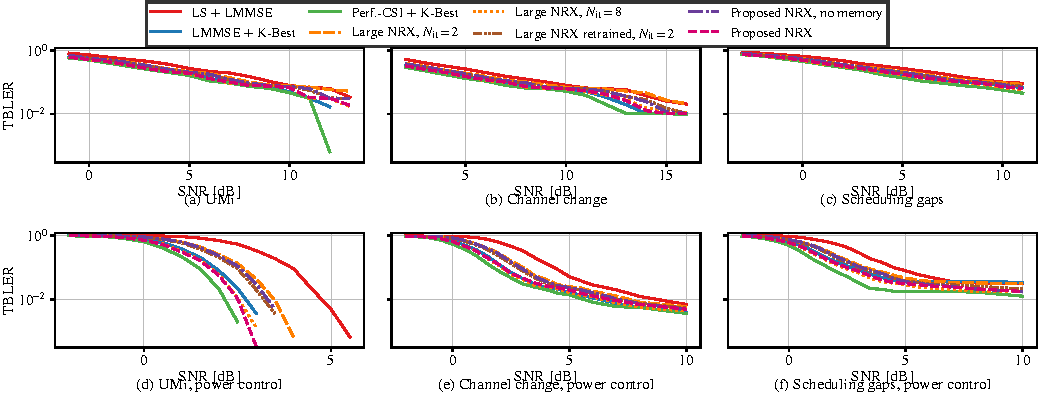
\includegraphics[width=\textwidth]{figures/tbler_vs_snr.pdf}
\caption{TBLER vs.\ SNR around a TBLER of 10\% for $U\times B\equiv 2\times 4$ MU-MIMO and MCS index $i=14$ without power control, (a)--(c), and with power control, (d)--(f). Dots mark the required SNR (Table~\ref{tab:required}); solid curves denote classical receivers.}
\label{fig:tbler}
\end{figure*}

\subsection{Training}
We train the proposed NRX in two stages on simulated TB sequences rather than independent slots. Sequences of 8 to 64 slots use 3GPP tapped delay line (TDL), urban microcell (UMi), and urban macrocell (UMa) channels~\cite{tr38901} with Doppler shifts up to 400\,Hz. They include near-far UEs, as well as scheduling gaps and channel changes, which expose the receiver to missing and outdated memory entries. In the first stage, we retrain the Large NRX with $N_{\mathrm{it}}=2$, starting from its released weights~\cite{wiesmayr2025realtime}. In the second stage, we add the pilot memory and the channel filter to this retrained NRX and continue to train its weights.

The loss is the binary cross-entropy of the LLRs plus, weighted by 0.01 as in the Large NRX, the mean squared error of the auxiliary channel estimate. In the first stage, the released Large NRX with $N_{\mathrm{it}}=8$ serves as a teacher~\cite{hinton2015distilling}, with equal weights on the transmitted bits and on its bit probabilities, which show the two-iteration NRX how reliably eight iterations detect each bit; the second stage uses no teacher. We use Adam~\cite{kingma2015} with a learning rate of $10^{-4}$ and 8 sequences per step, halve it when the validation TBLER, checked every $10^{3}$ steps, has not improved for two checks, and keep the best checkpoint, reached after $1.1\cdot 10^{4}$ and $6\cdot 10^{3}$ steps in the two stages.
\section{Evaluation}

\subsection{Simulation Setup}
We evaluate all receivers with Sionna~\cite{hoydis2022} for $U=2$ UEs and $B=4$ BS antennas, denoted $U\times B\equiv 2\times 4$, in the configuration of Wiesmayr et al.~\cite{wiesmayr2025realtime}: dual-polarized BS antennas with 3GPP TR 38.901 patterns~\cite{tr38901}, two omnidirectional antennas per UE with beamforming $\mathbf{v}=[1,1]^{\mathsf{T}}/\sqrt{2}$, 132 PRBs with 30\,kHz subcarrier spacing at 2.14\,GHz, modulation and coding scheme (MCS) index $i=14$ (16-QAM)~\cite[Table~5.1.3.1-1]{3gpp38214}, and PUSCH mapping type A with DMRS configuration type 1 and one additional DMRS position.

To reveal the effect of the memory, we simulate sequences of 64 consecutive slots (32\,ms) over continuously evolving channels, with 32 sequences for each of three conditions, each with a new random drop of outdoor UEs per sequence, Doppler shifts up to 400\,Hz, which corresponds to the maximum UE speed of 56\,m/s in the code release of Wiesmayr et al.~\cite{wiesmayr2025realtime}, and no path loss or shadow fading: \emph{UMi}, the 3GPP model with a fixed UE drop; \emph{channel change}, UMi with both UEs switching to a newly drawn channel at slot 33; and \emph{scheduling gaps}, UMi with a pool of four UEs, in which, in every slot, a scheduled UE is replaced with probability 0.25, the DMRS ports are redrawn with probability 0.25, and a UE pauses for up to four slots with probability 0.05.

We compare the proposed NRX with three classical baselines: LS + LMMSE, which uses LS channel estimation with linear interpolation and LMMSE detection; LMMSE + K-Best, which uses LMMSE channel estimation and K-Best detection~\cite{guo2006}; and Perf.-CSI + K-Best, which uses K-Best detection with perfect channel state information (CSI).\footnote{Covariance matrices for LMMSE channel estimation are computed per condition from separately simulated channels, and the K-Best detectors apply a list size of 64.} We also compare with the released Large NRX of Wiesmayr et al.~\cite{wiesmayr2025realtime}, trained on UMi channels only and evaluated with $N_{\mathrm{it}}\in\{2,3,8\}$; with the Large NRX retrained with $N_{\mathrm{it}}=2$, i.e., the result of our first training stage, whose validation TBLER had stopped improving and from which the proposed NRX starts; and with the proposed NRX with no memory, which has identical weights but empties the memory before every TB and thus operates on LS estimates. The LS + LMMSE and K-Best receivers are taken from the code release of Wiesmayr et al.~\cite{wiesmayr2025realtime}. All receivers use 20 belief propagation iterations for decoding.

We compute the TBLER over the TBs in slots 17 to 64, after the memory has filled, i.e., over 2{,}725 to 3{,}072 TBs per condition and SNR point. All receivers decode identical channels, payloads, and noise realizations. Except in the last tests with power control, we assume, as for DMRS bundling, that each UE keeps its phase continuous across slots, without carrier frequency offset, phase noise, or timing adjustment. As in the code release, the SNR is $E_b/N_0$.

\subsection{TBLER Performance}
Fig.~\ref{fig:tbler}(a)--(c) shows TBLER vs.\ SNR without power control. We call the SNR needed for a TBLER of 10\% the required SNR. Cutting the Large NRX from $N_{\mathrm{it}}=8$ to $N_{\mathrm{it}}=2$ costs more than 1\,dB in all three conditions, and retraining it with $N_{\mathrm{it}}=2$ recovers about half a dB. The proposed NRX requires 0.51 to 0.81\,dB less than this retrained Large NRX, from which it differs only by the pilot memory and the channel filter. It also outperforms the Large NRX with $N_{\mathrm{it}}=3$ in all three conditions, by 0.28 to 0.73\,dB, and stays within 0.20\,dB of the Large NRX with $N_{\mathrm{it}}=8$, although these differences rest on only a few UEs. With the retraining, the pilot memory and the channel filter thus substitute for more than one CGNN iteration, without trained weights.

The proposed NRX outperforms LS + LMMSE in all three conditions. LMMSE + K-Best, which requires the channel statistics, remains ahead of it for UMi and channel change, whereas the proposed NRX is ahead for scheduling gaps. Perf.-CSI + K-Best remains ahead of all other receivers.

In contrast to the waterfall curves of Wiesmayr et al.~\cite{wiesmayr2025realtime}, TBLER decreases slowly with SNR for all receivers, because with a fixed beamformer and no power control, some UEs have low channel power; after the channel change, the new channel of one UE is about 18\,dB weaker than the median. Against the effective SNR, i.e., the SNR plus the mean power of the UE's effective channel over its TB in dB, the proposed NRX requires 0.58 to 0.90\,dB less than the retrained Large NRX and stays within 0.20\,dB of the Large NRX with $N_{\mathrm{it}}=8$.

\subsection{Benefit of the Pilot Memory}
Comparing the proposed NRX with its no-memory version, which operates on LS estimates, isolates the memory. The memory reduces the required SNR in all three conditions, by 0.70 to 0.78\,dB. Without its memory, the proposed NRX requires up to 0.19\,dB more than the retrained Large NRX, as its weights are trained for the refined estimates. The gain stems from the earlier slots: if the channel filter predicts every pilot from the current TB only, with its weights still fitted on the memory and with the first-order model, the proposed NRX requires 0.02 to 0.19\,dB more than with its memory emptied, i.e., on the LS estimate of the nearest pilot.

The gain of the memory grows with the Doppler shift: in effective SNR for UMi, it rises from 0.55\,dB at Doppler shifts below 50\,Hz to 0.94\,dB above 175\,Hz, as the entries mainly average the noise of the LS estimates on slow channels, whereas on fast channels the newest entry adds estimates before the first DMRS symbol of the current slot.

On two further datasets at a fixed SNR, which add TDL and UMa channels, closely spaced line-of-sight (LOS) UEs, near-far UEs, and, on one dataset, channels ray-traced with Sionna RT~\cite{hoydis2023}, the memory lowers TBLER in 16 of the 17 cases, and the proposed NRX outperforms the Large NRX with $N_{\mathrm{it}}=8$ in 6 cases, for both TDL channels and the UMa channels on both datasets, which it does not without its memory. The Large NRX with $N_{\mathrm{it}}=8$ remains ahead in 10 cases, most clearly for closely spaced LOS and near-far UEs.

The pilot memory and the channel filter do not depend on the NRX. Replacing the LMMSE channel estimation of LMMSE + K-Best, they reduce its required SNR by 0.15 to 0.43\,dB. For comparison, we extend this LMMSE estimation to the DMRS symbols of all stored TBs, up to seven, with the correlation across slots measured on separately simulated channels. This classical estimator trails the channel filter by 0.06 to 0.09\,dB for UMi and scheduling gaps and by 0.80\,dB for channel change, where it even falls 0.56\,dB behind LMMSE + K-Best, as the channel statistics cannot reveal when the channel of a UE changes.

\subsection{Power Control}
Without power control, most errors occur on UEs whose channel power stays low, and a network raises the transmit power of such UEs. We therefore also evaluate all receivers with closed-loop power control as in 5G NR~\cite{3gpp38213}: after each slot in which a UE is scheduled, the BS measures its received power, which we assume exact, and sends an accumulated transmit power control (TPC) command of $-1$, $0$, $+1$, or $+3$\,dB toward the nominal received power, at which the SNR is defined. The UE applies it in its next scheduled slot, within $-10$ to $+15$\,dB of its nominal power. Channels, payloads, noise, and receivers are those of Fig.~\ref{fig:tbler}(a)--(c), and the memory entries are not rescaled by the TPC commands.

In Fig.~\ref{fig:tbler}(d)--(f), the proposed NRX requires 0.51 to 0.71\,dB less than the retrained Large NRX and 0.36 to 0.51\,dB less than the Large NRX with $N_{\mathrm{it}}=3$. It stays within 0.17\,dB of the Large NRX with $N_{\mathrm{it}}=8$, is on par with it for UMi, and outperforms LMMSE + K-Best in all three conditions. The memory contributes 0.63 to 0.80\,dB. Power steps may also break phase continuity. With a uniformly random phase jump at every power step, the memory still contributes 0.64 to 0.81\,dB, and on each UE's first three TBs after a jump, the proposed NRX fails less often than the retrained Large NRX in all conditions. On the TB of a channel change or a phase jump, the channel filter uses no stored TB for more than 90\% of the UEs' DMRS symbols, and otherwise for less than 1\%. With a frequency offset of $\pm 0.1$\,ppm per UE, the most 3GPP allows~\cite{3gpp381011}, the proposed NRX loses less than 0.1\,dB and the retrained Large NRX about 0.15\,dB, as the channel filter tracks the rotation. With the TDD pattern DDDSU, i.e., one uplink slot every 2.5\,ms, the memory keeps more than 70\% of its gain, or at least 0.6\,dB if the eight-slot limit counts uplink slots, and the proposed NRX still leads the retrained Large NRX by at least 0.4\,dB.

\subsection{Other Modulations}
For QPSK (MCS 9) and 64-QAM (MCS 19), we train and evaluate all NRXs in the same way, starting from the released weights for each MCS; Fig.~\ref{fig:modulations} compares them at all three modulations. With QPSK and 64-QAM, the memory contributes 0.7 to 1.1\,dB, and the proposed NRX outperforms the retrained Large NRX and the Large NRX with $N_{\mathrm{it}}=3$ in all cases, with and without power control. With QPSK, it also outperforms the Large NRX with $N_{\mathrm{it}}=8$ in all cases; with 64-QAM, it stays within 0.15\,dB of it with power control, but trails it by about 0.7\,dB after scheduling gaps without power control. LS + LMMSE needs at least 0.8\,dB more with 64-QAM and 2.3\,dB more with QPSK.

\begin{figure}[!t]
\centering
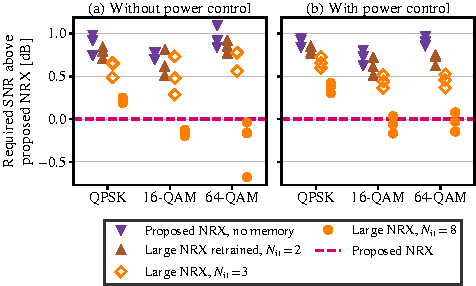
\includegraphics[width=\columnwidth]{figures/modulations_summary.pdf}
\caption{Required SNR of the stateless NRXs relative to the proposed NRX (dashed line) for QPSK, 16-QAM, and 64-QAM, without and with power control. Each marker is one test condition.}
\label{fig:modulations}
\end{figure}

\subsection{Latency}
As in Wiesmayr et al.~\cite{wiesmayr2025realtime}, we time the network from the received slot and LS estimate to the LLRs with TensorRT~10.3 in FP16 and batch size one, without decoding and host-device transfers, and export every NRX as in their code release. We report the median of 2{,}000 runs on an NVIDIA A100 GPU. The Large NRX with $N_{\mathrm{it}}=2$ takes 0.79\,ms, and each further CGNN iteration adds 0.28\,ms. Thus, $N_{\mathrm{it}}=2$ meets the 1\,ms budget, which $N_{\mathrm{it}}=3$ exceeds (1.07\,ms).

For the proposed NRX, CUDA kernels apply the channel filter before the TensorRT engine of the two CGNN iterations. The filter weights and the memory's contribution only depend on earlier slots and are computed before the slot arrives, in 0.11\,ms for both UEs. The proposed NRX takes 0.81\,ms, and the GPU work per slot including this computation is 0.91\,ms, or 0.88\,ms if it runs at the same time as the slot, so it meets the 1\,ms budget either way.
\section{Conclusion}
We have presented a stateful NRX for 5G NR PUSCH whose channel filter, fitted and not trained, uses a pilot memory of LS channel estimates without labels or decoder feedback. With two CGNN iterations and QPSK, 16-QAM, or 64-QAM, it outperforms stateless NRXs with up to three iterations and performs close to the eight-iteration NRX, with and without power control, while it remains real-time capable, unlike the three-iteration NRX. Future work includes measured data.

\bibliographystyle{IEEEtran}
\bibliography{references}

\end{document}
